\chapter{Control Design and Development}



\section{Static Controller} \label{NeuralController}

The development of the controller, inspired by the methodologies proposed in the paper \cite{QSC}, aims to determine the optimal muscle excitation to stabilize the wrist's position. The architectural layout of this controller is portrayed on Figure \ref{fig:BDC}.

The input of the controller is the desired arm configuration. Using the Inverse of the Arm Statics model, described in Section \ref{sec:model}, the required torques to maintain the arm in a static position are computed. These torques are subsequently given as an input into the Muscle Torque Production model, elaborated in Section \ref{sec:model}. This model outputs the corresponding muscle excitations which will define the neural excitation input for the Dynamic Arm Simulator. 

The Dynamic Arm Simulator will then determine the arm's dynamics in accordance with the Rosenbrock equation, as explained in Section \ref{sec:dynamics}. Post these dynamic computations, the wrist's actual position is deduced. The error between the desired and the actual wrist position will drive a PID Controller, which will calculate the corrective force needed to match the desired wrist position. The kinematic Jacobian, Section \ref{sec:torque}, will compute the requisite corrective torque. This torque, when combined with the desired torque from the Inverse Arm Statics, provides the total torque which is then input to the Inverse Muscle Torque model, closing the control loop. 


\begin{figure}[h!]
    \centering
    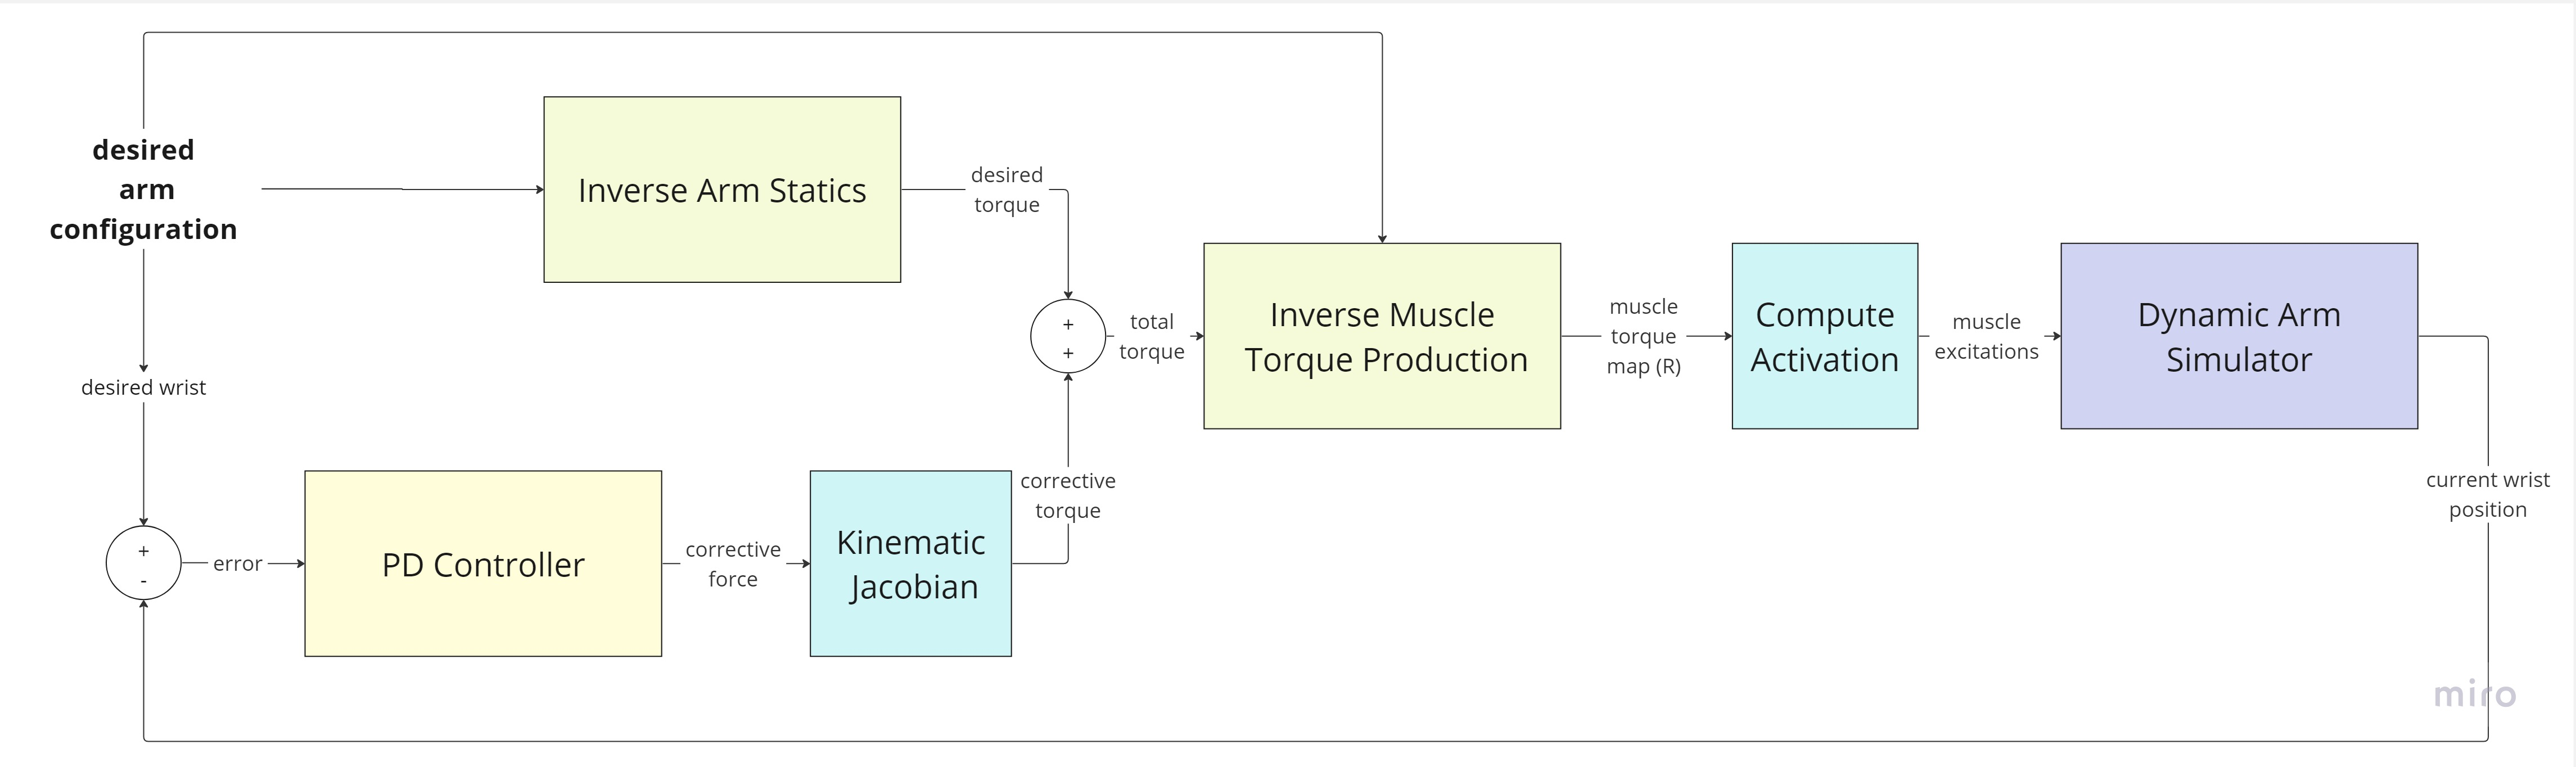
\includegraphics[width=1\textwidth]{Pictures/Controller/controller-diagram.jpg}
    \caption{Controller Block Diagram inspired in \cite{QSC}}
    \label{fig:BDC}
\end{figure}

\subsubsection{PD-Tuning}
To assure the PID Controller's performance, an exhaustive hand-tuning was undertaken across 20 different positions, concluding in values of \(K_p = 300\) and \(K_i = 100\). \(K_d = 0\) resulting in only a PD. 

\subsection{Predicting Static Torque}
static_torque = predict_static_torque(desired_arm_config)';
desired_torque = torque_feedback+static_torque;
TotalTorque(i,:)=desired_torque;
if mod(i,10)==0
    alpha0 = compute_neural_excitation(desired_arm_config, ...
        desired_torque,alpha0);
    for m=1:8
        mus=whichMuscles(m);
        u(mus)=alpha0(m)*1;
    end            
end

\subsection{Predicting Muscle Excitations}\label{computemuscleexcitation}

In muscle-driven systems, accurately determining muscle activation patterns is crucial for understanding force generation. The provided functions aim to compute optimal muscle activations under given constraints using the penalty method and a quasi-Newton optimization approach. This method is inspired by \cite{QSC}.

The objective is to compute the muscle activation \texttt{act} for given muscle-torque relationships \texttt{M}, desired torques \texttt{tau}, and initial guesses for activations \texttt{alpha0}.

The muscle-torque relationships \texttt{M} the Muscle Torque Production model hyperparameters calculated following the steps explain in Section \ref{sec:model}. This outputs a matrix each column represents the torque about the shoulder elevation plane, shoulder elevation, shoulder rotation adn elbow flexion produced by each muscle group. 

\subsection{Methodology}
\begin{description}
    \item[Objective:] Solve the equation \( M \cdot \alpha = \tau \) for the muscle activations \( \alpha \).
    \item[Broyden's Quasi-Newton Method:] This iterative optimization technique is employed to approximate the solution of the equation. It starts with an initial guess and updates it based on a Broyden approximation to the inverse Jacobian matrix.
\end{description}

\subsection{Output Constraints}
Ensure activations are non-negative and normalized such that the maximum activation does not exceed 1.

\section{Armijo Rule: \texttt{armijo}}

\subsection{Overview}
Determines the optimal step size (or learning rate) during iterations, ensuring a sufficient decrease in the function value.

\subsection{Methodology}
Using a backtracking approach, the step size \texttt{alpha1} is repeatedly halved until the sufficient descent condition is met.

\section{Penalty Function: \texttt{penaltyFunc}}

\subsection{Overview}
Imposes penalties on undesired muscle activations, such as negative values or values greater than one.

\subsection{Methodology}
\begin{description}
    \item[Objective Function:] Consists of three main components:
    \begin{enumerate}
        \item Quadratic norm of activations.
        \item Quadratic difference between desired and actual torques scaled by a factor \( c \).
        \item Penalty \( K \) for activations outside the [0,1] range scaled by a factor \( c2 \).
    \end{enumerate}
    \item[Gradient Computation:] Gradient of the objective function w.r.t. activations.
\end{description}

\section{Conclusion}

The \texttt{computeActivation\_Nuri} function, supported by the Armijo rule and a penalty-based approach, effectively computes the muscle activations while ensuring feasible values. By employing the quasi-Newton method, the function efficiently converges to the optimal solution, providing a robust mechanism for muscle-torque simulations in biomechanical systems.
            

\subsection{Feasible Points}
With this tuned controller, a grid, encompassing 960 points, was generated using the \textbf{create\_grid} function (refer to Section \ref{sec:tp}). Each point's arm configuration was calculated using the PI force controller, as detailed in Section \ref{sec:PI}. The feasibility of a point was determined by the ability of the controller to sustain for 1 second its position with an error margin of 0.1. For clarification purposes, the start and the goal position of the controller are set to be the same. 
For seamless and accurate operations, a time step (\(t_{step}\)) of 0.001 is employed. To improve the controller's stability an auxiliary force is exerted on the arm in the first 100 steps. This eliminates potential oscillations and assures a better control performance.

The figures (gif if opened in Adobe Acrobat) below present the generated grid. Points in red signify positions where the controller failed to find the neural excitation needed to sustain for 1 second. In contrast, green points indicate successful stabilization by the controller. These feasible points will be used in the following section (Section \ref{sec:path}) to generate paths for the arm to follow. 


\begin{figure}[ht]
    \centering
    \animategraphics[autoplay,loop,width=0.8\textwidth]{12}{Pictures/Controller/gif/feasiblepoints-}{0}{149}
    \caption{Feasible points. Open in Adobe Acrobat to see gif movement.}
    
\end{figure}
\section{Path Following Quasi-Static Controller Development } \label{sec:path}

The goal is to develop a controller that allows the dynamic arm  to navigate or follow a specific trajectory or path. This will simulate the rehabilitation reaching task to be performed. For more information on rehabilitation tasks refer back to Section \ref{rehabilitation_task}. Quasi-static control allows to design a safe, precise and movement-controlled therapy, as it focuses on slow, steady and controlled operations. It facilitates the decomposition of the entire reaching path trajectory into smaller static positions. Dividing the task into smaller steps offers some benefits under the rehabilitation lens:
\begin{itemize}
    \item \textbf{Gradual Progression}. Rehabilitation often demands gradual approach towards exercises, specially for recovering patients. progress.
    \item \textbf{Progress Tracking} Breaking the movement into smaller steps helps not only patients to progress at a comfortable and safe pace but allows to keep track of the progress.
    \item \textbf{Minimized Fatigue} Continuous motions can take a toll in patients with limited strength and endurance. Smaller tasks reduce muscle and join strain preventing fatigue. Using a quasi-static controller can help modify the parameters to adjust to the patient's abilities. 
\end{itemize}

For a clearer understanding of the quasi-static control designed, refer to the flow diagram included in this chapter (Figure \ref{fig:PathController}). Here’s a descriptive step-by-step breakdown of the process of path controller:

\begin{enumerate}
    \item \textbf{Selection of Target Position}: From a set of feasible points, a target position is chosen. This serves as the end-point or goal for the system.
    
    \item \textbf{Path Discovery via the 'find path' Function} (see Section \ref{findpath}, for a more detailed explanation of the function): The selected target position is input into the 'find path' function. This function works by first identifying the nearest neighbors from the feasible points workspace. Among the first 200 nearest neighbors of the starting point, it selects one that:
    \begin{itemize}
        \item Is at a distance \(d = 4\) units away from the starting point. This distance recommendation comes from the paper \cite{QSC}.
        \item Lies in the direction of the end-point or target position.
    \end{itemize}
    Through this method, a path consisting of multiple positions is generated.
    
    \item \textbf{Setting Initial Simulation Parameters}: At the beginning of the simulation, the initial position from the path is defined. Moreover the simulation parameter are set: \(t_{step} = 0.003\), and a $frequency$ of 30Hz. The variable $frequency$ refers to the rate at which the FES (Functional Electrical Stimulation) device can change its input. This is a criteria detailed on the design Section \ref{Design} limited by the FES devices.
    
    \item \textbf{Control Loop}: The control loop operates as previously outlined in the Section \ref{NeuralController} , with a few distinct modifications:
    \begin{itemize}
        \item \textbf{Neural Excitation}: This only takes place at set intervals based on the defined $frequency$.
        \item \textbf{Position Switching}: At every $time_{switch}$ the position in the control system is updated to the subsequent one in the predefined path array.
        
        If the hand has not reached the vicinity of the targeted position within the set time frame of $time_{switch}$, the system will attempt to reach the position a maximum of two more times before potentially moving to the next point or terminating.
    \end{itemize}
\end{enumerate}

In conclusion, the proposed controller is designed to guide a dynamic arm through specified trajectories, mimicking the rehabilitation reaching tasks outlined in Section \ref{rehabilitation_task}. Quasi-static control is used to emphasize safety, precision and control, three key components for a successful rehabilitation. Key components of the control system presented include a \textbf{\textit{find\_path} }function that uses KNN to find the best positions that will define the path to the desired target. Moreover the control loop, adapted from the one on Section \ref{NeuralController}, operated with timed neural excitation (controlled by the variable $frequency$) and position switching to guide the arm accurately along the predefined path (controlled by variable $time_{switch}$).


\begin{figure}[h!]
    \centering
    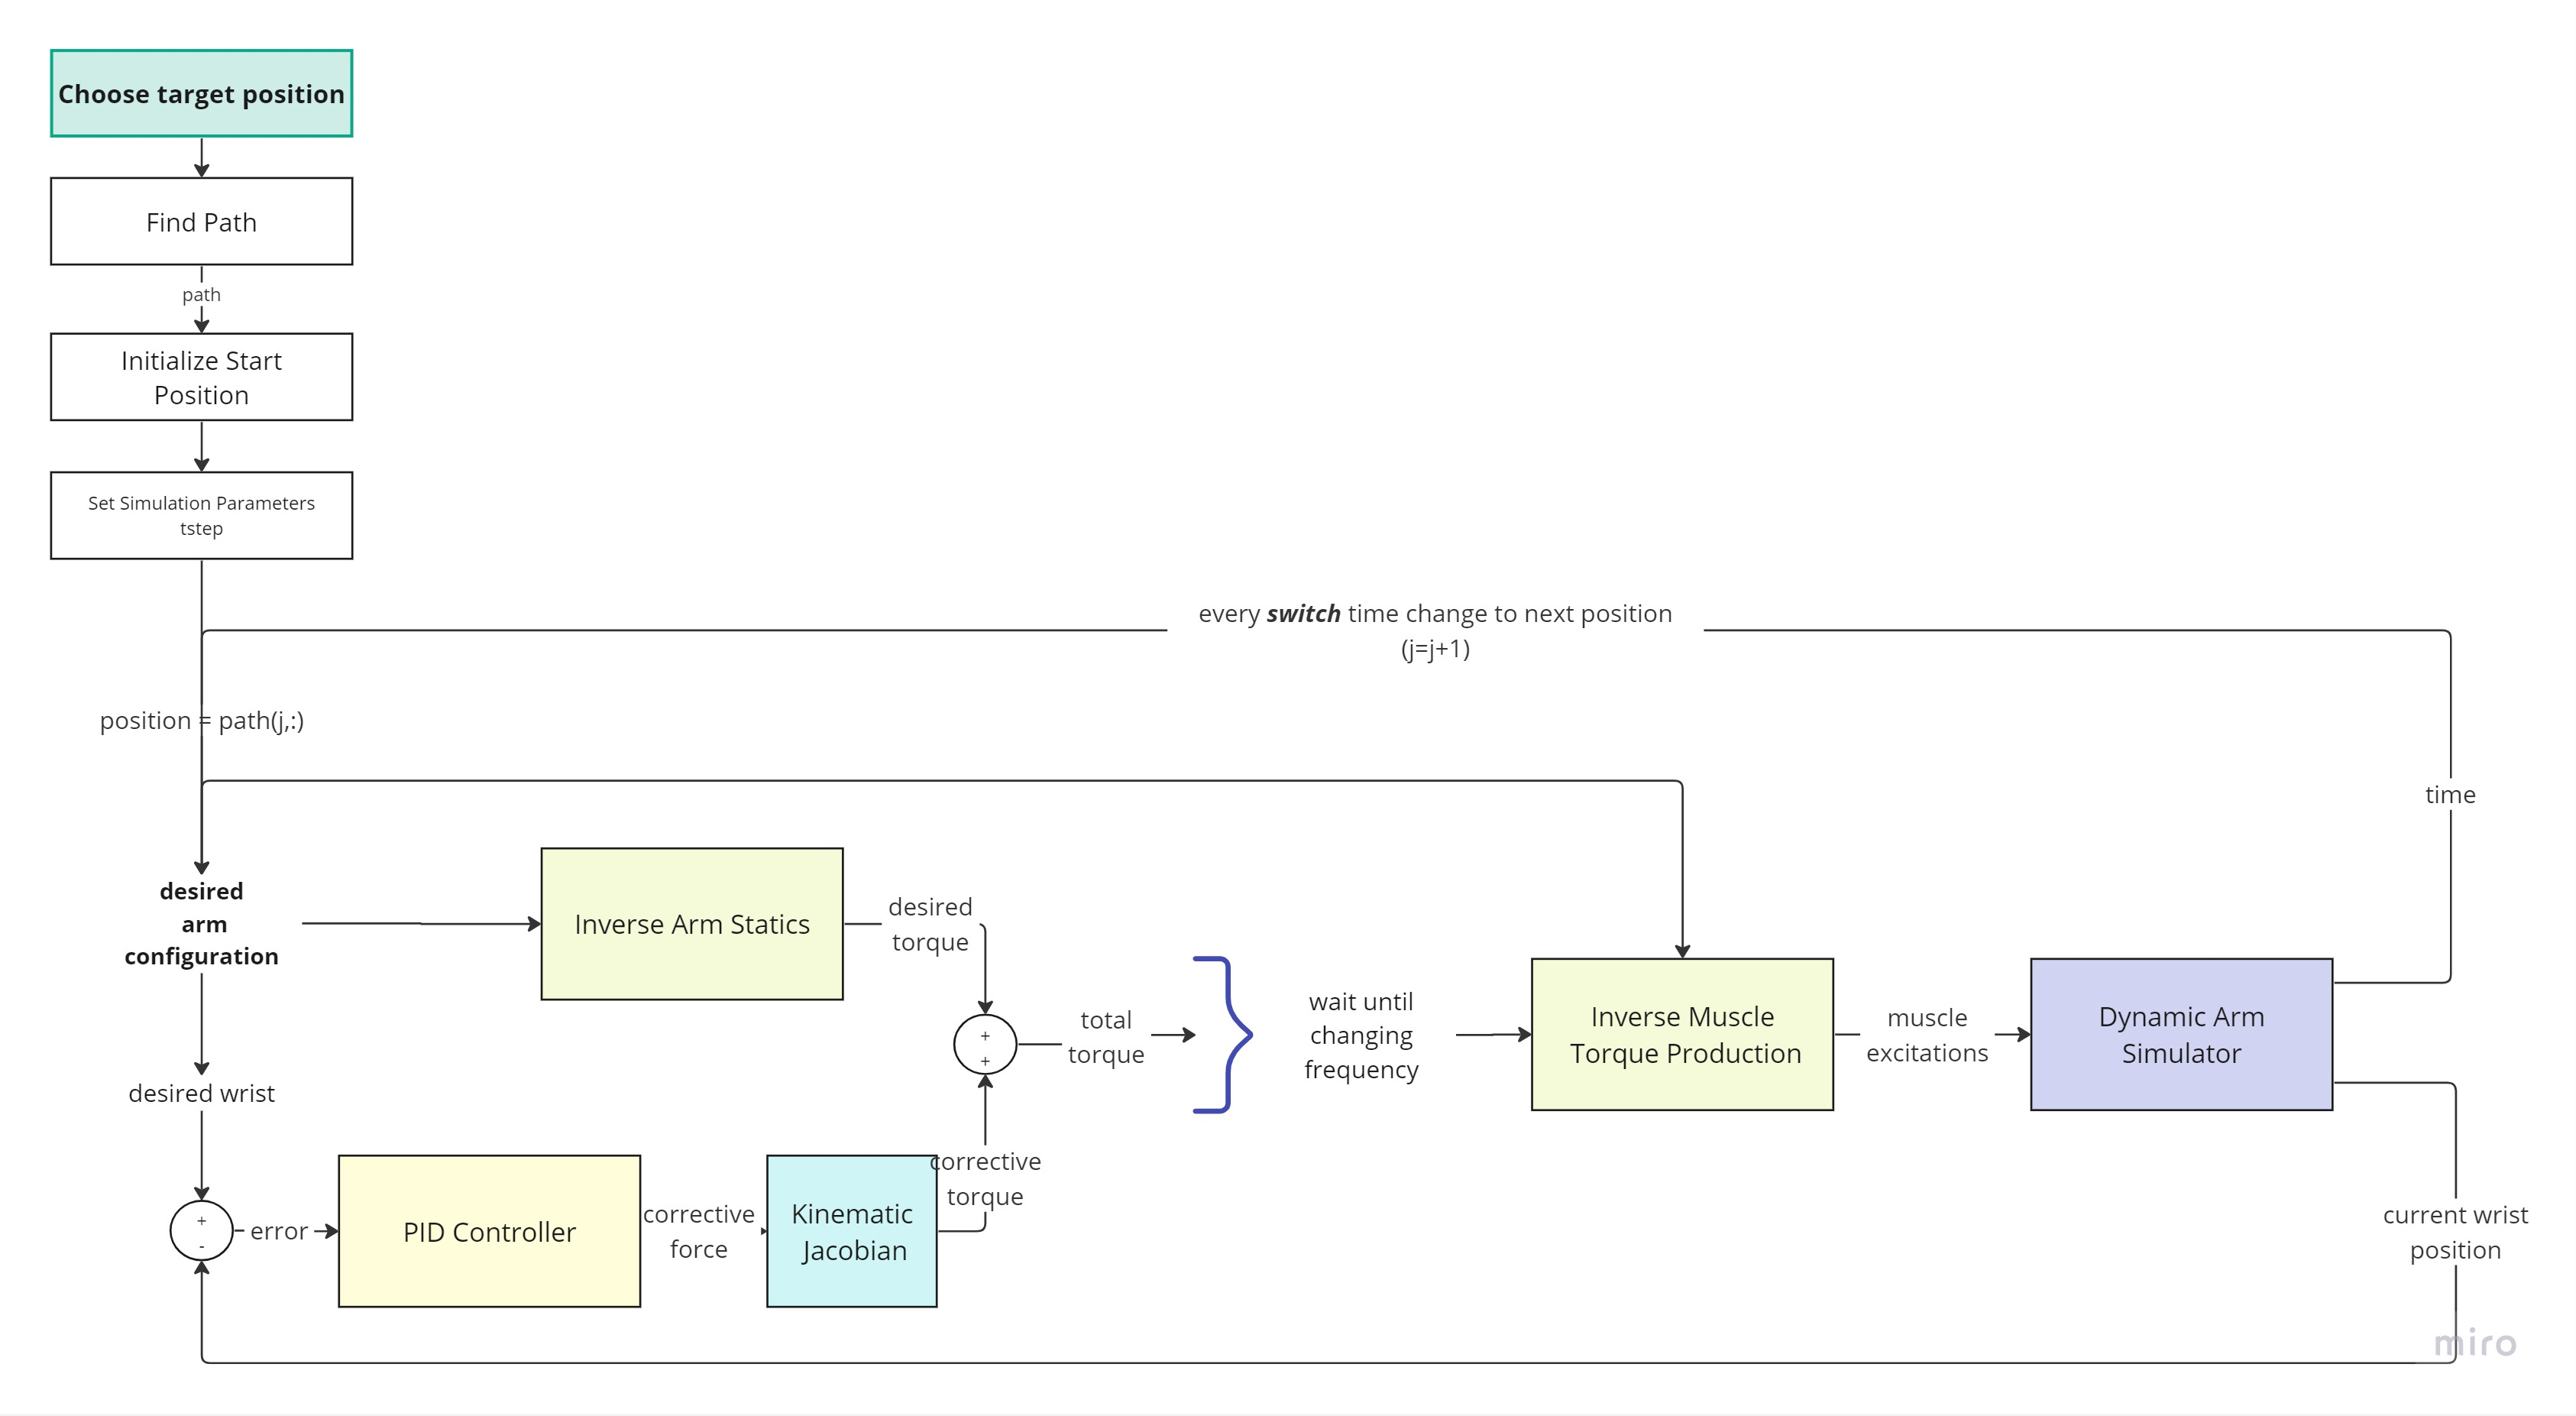
\includegraphics[width=1\textwidth]{Pictures/Controller/Quasi-Static Path Controller.jpg}
    \caption{Flow Diagram Quasi-Static Path Controller }
    \label{fig:PathController}
\end{figure}

\subsection{Find Path Function} \label{findpath}

The \texttt{FindPath} function calculates a path between two positions within a predefined set of feasible wrist points. The function takes three input parameters: $d$,  $startPos$ and $endPos$. 

The code will load a file that contains all the feasible wrists positions to calculate a path from. Section \ref{NeuralController} explains how the feasible positions are determined. 

Once all the initial parameters are set, the function begins to construct the path. K-Nearest Neighbours is the supervised machine learning algorithm used to calculate the most optimal path. The Matlab function \textbf{knnsearch} is used to seek the predefined number of nearest neighbours to the current position within the feasible positions. Then, another \textbf{knnsearch} is performed to identify which one of the closest neighbours is closer to the end position. The selected point should be within a distance $d$ from the current position but closet to the end position.

This process is repeated until the path reaches the desired end position. As a result, find path outputs an array called path will all the positions.


\begin{figure}[h!]
    \centering
    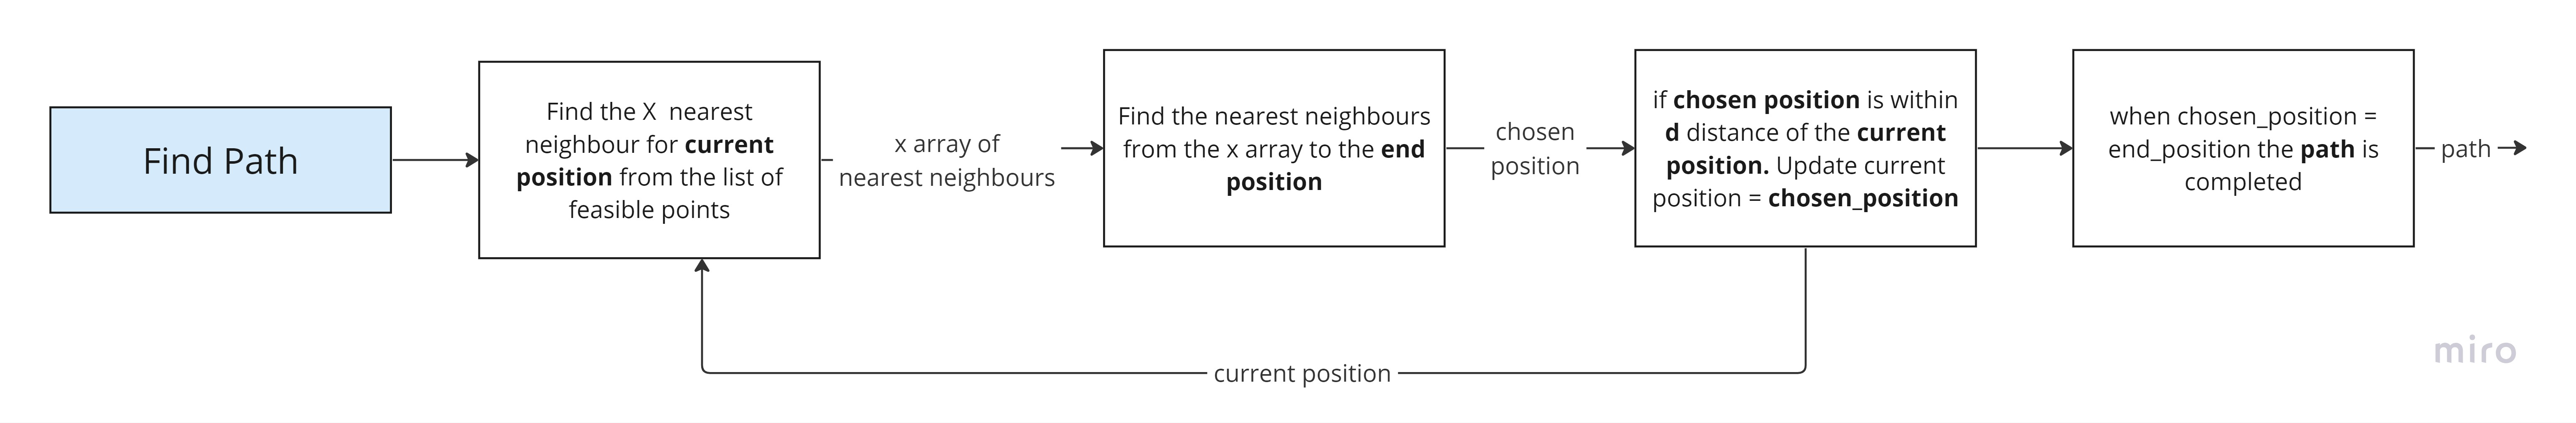
\includegraphics[width=1\textwidth]{Pictures/Controller/findpath.jpg}
    \caption{Flow Diagram Find Path Function }
    \label{fig:FindPath}
\end{figure}


\newpage
\section{EMG-Influenced Controller Development}

Building on top of the controllers previously designed and discussed in this section, we further extend our investigation into the intricate challenges faced by stroke patients. An after-math of stroke is the muscular imbalances, most specifically muscle spasticity, which refers to muscle stiffness that influences movement and speed. As a result, they present difficulty extending the arm. The biceps tend to be over-activated and the triceps and anterior deltoid under-activated \cite{IOL}. To counteract these muscular imbalances, this controller has being design to simulate an effective and targeted electric stimulation. 

Two key additions are included in the following controller design:

\begin{enumerate}
    \item a component that emulates the over activity of the biceps post-stroke 
    \item the addition of FES to activate the triceps
\end{enumerate}

A complete flow diagram is portrayed on Figure \ref{fig:FESController}

\subsection{Emulating Biceps Over-Activity}

The code segment initiates by calculating muscle activation levels using the \textbf{\textit{computeActivations}} function, which factors in muscle force models and desired torques  (refer to Section \ref{NeuralController}). Then, it proceeds to iterate through the set of  muscles. When the loop reaches the fifth muscle, the biceps, the activation level of the biceps is modulated by a factor termed \textbf{\textit{stroke}}, representing the over-activity induced due to the stroke condition. This modulation is subsequently bounded: if the resultant activation surpasses a threshold of 1, it is capped at this upper limit. In scenarios where the activation is null and the stroke factor exceeds 1, a minimal activation level of 0.3 is set to ensure a base activation. For each iteration, the modified activation values are assigned to the corresponding muscle index in the control input vector u. It is important to highlight that the values are only updated with respect to the FES frequency (concept explained in Section \ref{sec:path}).

\subsection{FES Stimulator for the Triceps}

Considering the biomechanical implications, this project focuses on applying the Functional Electrical Stimulation the triceps. The control examines the triceps activation levels. This information comes from the Dynamic Arm Simulator and in a real case scenario it will come from EMG sensors situated in the triceps of the human. 

If no activation is detected, a default minimal value is assigned. However, in cases with existing activation, a sigmoid-based control system is adopted. 
\begin{equation}
    \sigma(z) = \frac{1}{1 + e^{-z}}
\end{equation}

This methods adapts the gain in a smooth manner between predefined boundaries, allowing for a nuanced control response that remains sensitive to the velocity-driven nature of spasticity.

For correct simulation it is ensured that the triceps activation remains bounded between [0.2, 1]. 


\newpage
\begin{landscape} % Start landscape page
  \begin{figure}[h!]
    \centering
    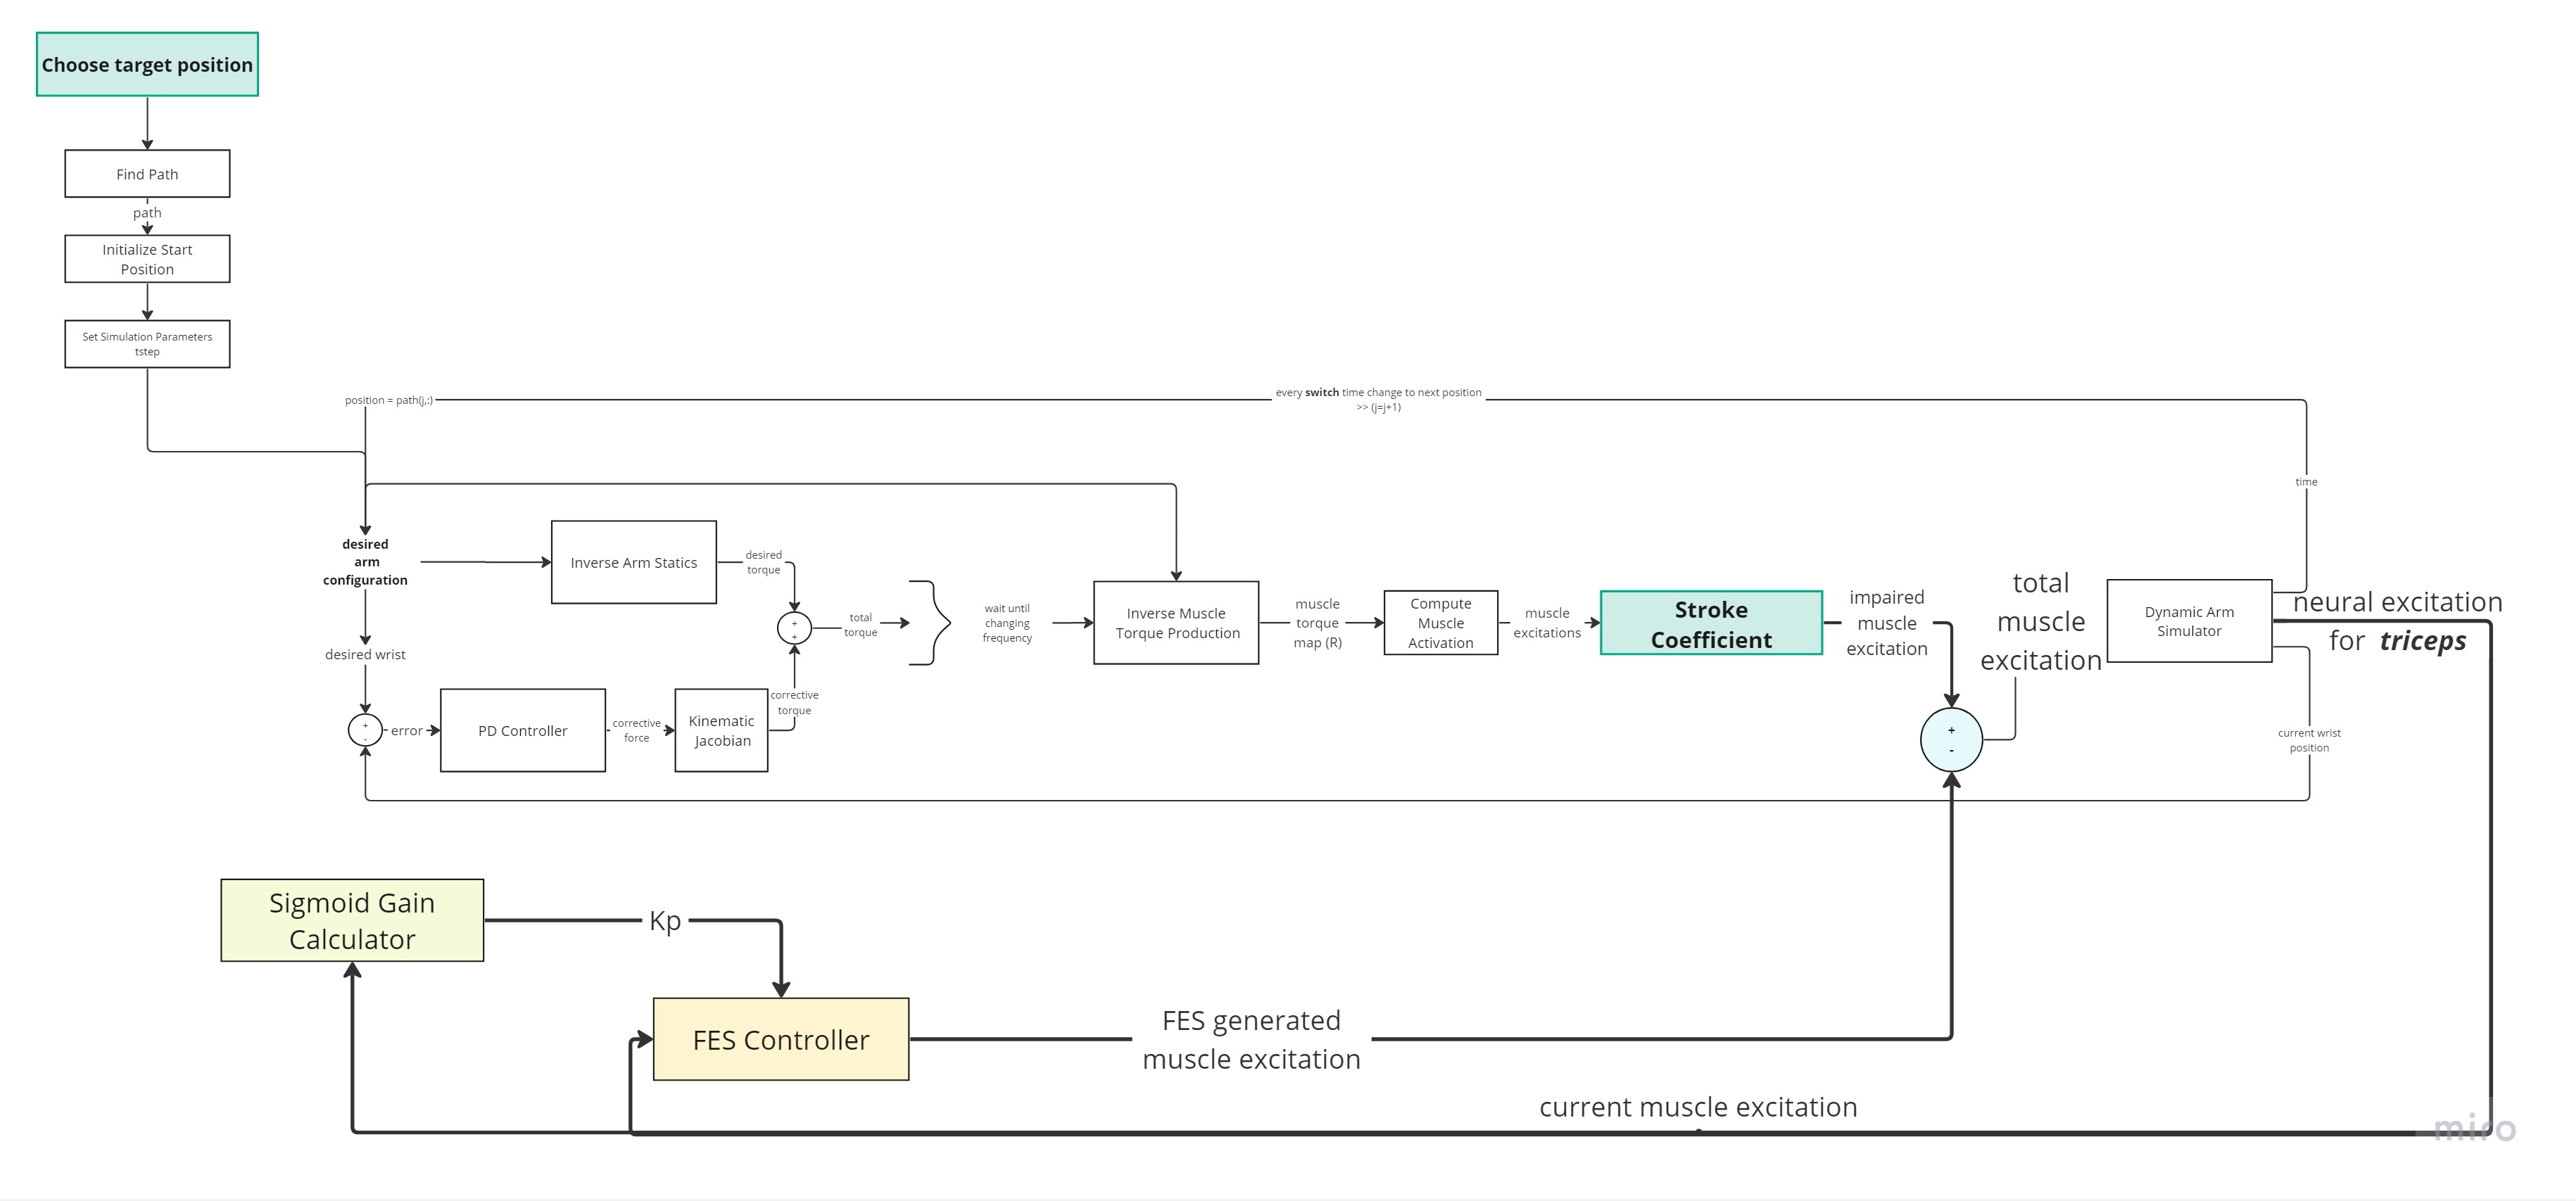
\includegraphics[width=1.7\textwidth]{Pictures/Controller/FESController.jpg} % Replace "filename.jpg" with the name of your image file
    \caption{Flow Diagram for EMG-influenced FES Controller} % Optional caption
    \label{fig:FESController} % Optional label for referencing
  \end{figure}
\end{landscape} % End landscape page

\subsection{P Controller Tuning: Simulated Annealing}